Como visto no capítulo anterior \ref{chapter:bibliotecas_do_ruby_e_segurança}, a maior parte das bibliotecas do
\emph{Ruby} são distribuídas na forma de \emph{gems}, e também vimos na seção
\ref{subsection:o_programa_gem} deste mesmo cápitulo que a ferramenta \emph{gem} é um sistema de distribuição
sinilar ao  \emph{\href{https://packages.qa.debian.org/a/apt.html}{apt-get}}, que facilita o compartilhamento e a
instalação de \emph{gemas}.

Deste modo, como já temos alguns conhecimento básicos sobre bibliotecas e sobre o \emph{Ruby}. Este cápitulo
tem o objetivo de mostrar um passo-a-passo que pode ser seguido para criar uma gema.

%A ideia de criar uma gema, geralmente vai surgir quando se perceber que uma determinadade funcionalidade
%é utilizada frequentemente nos sistemas que a equipe trabalha.
% (\emph{Ctrl + C}, \emph{Ctrl + V}).

Inicialmente, antes de iniciar o processo de criação de uma gema, precisamos entender para que serve cada um
de seus compoentes, e isso será explicado logo a seguir na seção \ref{section:estrutura_de_uma_biblioteca_do_ruby}.
Depois com o conhecimento de cada componente da gema, apresentaremos um modelo de criação de gemas
na seção \ref{section:modelo_de_criação}. Caso tenha dúvidas sobre as ferramentas utilizadas ou de como preparar
o ambiente de desenvolvimento, pode-se consultar os apêndices \ref{chapter:ferramentas_utilizadas} ou
\ref{chapter:preparação_do_ambiente}, respectivamente.


\section{Estrutura de uma Biblioteca do Ruby}
\label{section:estrutura_de_uma_biblioteca_do_ruby}

Uma gema do \emph{Ruby}, obrigatoriamente deve possui um nome, um número de versão e uma plataforma.
Internamente ela deve possuir códigos de funcionalidade, uma documentação e um \emph{\textbf{gemspec}}.

A sua estrutura geralmente é organizada em 3 arquivos bases: o \emph{\textbf{gemspec}}, o
\emph{\textbf{Rakefile}} e o \emph{\textbf{README}}, e em 3 diretórios principais: \emph{\textbf{bin}},
\emph{\textbf{lib}}, e \emph{\textbf{test}} ou \emph{\textbf{spec}}. Na listagem abaixo veremos para que
serve cada um destes arquivos e diretórios.

\begin{itemize}

 \item O \emph{\textbf{gemspec}} é um arquivo do tipo ‘‘\emph{.gemspec}'' que possui as informações básicas
 de uma gema, como por exemplo o seu nome, sua descrição, seu autor, seu endereço, e suas dependências.

 \item O \emph{\textbf{bin}} é um diretório que possui os arquivos executáveis da gema que serão
 carregados quando a gema for instalada.

 \item O \emph{\textbf{lib}} é um diretório que possui todos os códigos \emph{Ruby} referentes ao
 funcionamento da gema.

 \item O \emph{\textbf{test}} ou \emph{\textbf{spec}} é um diretório que possui todos os códigos \emph{Ruby}
 de testes. Eles podem ser executados manualmente ou por meio do \emph{Rakefile}.

 \item O \emph{\textbf{Rakefile}} é um arquivo que possui código \emph{Ruby} que faz a otimização de algumas
 funcinalidades por meio da execução do programa \emph{\href{https://github.com/jimweirich/rake}{rake}}
\footnote{rake: \url{https://github.com/jimweirich/rake}}. Um exemplo, é a execução de todos os arquivos
de testes do diretório \emph{test} ou \emph{spec}.

 \item O \emph{\textbf{README}} é um arquivo que usualmente possui a documentação da gema. Esta
 documentação, usualmente é retirada de comentários que estão dentro do código, e gerados automaticamente
 quando a gema é instalada. A maioria das gemas possuem a documentação
 \emph{\href{http://rdoc.sourceforge.net/doc/}{RDoc}} \footnote{RDoc: \url{http://rdoc.sourceforge.net/doc/}},
 e as outras, em menoria, possuem a documentação \emph{\href{http://yardoc.org/}{YARD}}
 \footnote{YARD: \url{http://yardoc.org/}} [\citeonline{guide_what_is_a_gem_rubygems}].

\end{itemize}


\section{Modelo de criação}
\label{section:modelo_de_criação}

O primeiro passo para se criar uma gema, é construir uma solução de um certo problema que será utilizado
com frequência. Por exemplo, a função que calcula a raiz quadrada de um número, é uma funcionalidade que
usualmente utilizamos quando estamos fazendo cálculos.

Após encontrar uma ideia para a criação de uma gema, deve-se elaborar um projeto, fazendo o levantamento
de requisitos, o \emph{design}, a implementação, os testes e a entrega.

Por simplificação, nesta seção somente apresentaremos a parte de implementação do modelo de criação de uma
gema, mas nunca se deve esquecer de seguir todos os passos de um projeto, desde o momento da formação da
ideia até a sua entrega. Caso esses passos não sejam seguidos, existem altos riscos de se perder recursos,
como tempo e dinheiro.

Para facilitar a apresentção deste modelo utilizaremos como exemplo a gema
\emph{\href{https://github.com/toshikomura/gemtranslatetoenglish/tree/without_path}{gemtranslatetoenglish}}
\footnote{gemtranslatetoenglish : \url{https://github.com/toshikomura/gemtranslatetoenglish/tree/without_path}},
que tem como objetivo fazer a tradução de um texto em português para um texto em inglês.

Futuramente pretendemos aumentar o vocabulário da gema de exemplo, mas até o momento de término deste
trabalho, ela possuía somente a tradução de duas palavras, ‘‘\emph{OI}'' para ‘‘\emph{HELLO}'' e
‘‘\emph{MUNDO}'' para ‘‘\emph{WORLD}''. Apesar de possuir pouco vocabulário, a gema ‘‘\emph{gemtranslatetoenglish}''
possui características suficientes para a aparesentação do tutorial deste trabalho.

Nesta seção, apresentaremos primeiramente como se pode criar uma estrtura básica de uma gema na sub-seção
\ref{subsection:criando_a_estrutura}, em seguida mostraremos na sub-seção \ref{subsection:gemspec} como
se deve editar o arquivo \emph{.gemspec}, depois iremos apresentar como se pode desenvolver o código
de funcionalidades de uma gema na sub-seção \ref{subsection:codigo_de_funcionalidade_no_diretorio_lib},
sequêncialmente apresentaremos na sub-seção \ref{subsection:codigo_de_teste_no_diretorio_test_ou_spec} como
implementar o código de testes, em seguida na sub-seção \ref{subsection:execução_de_testes} apresentaremos
uma forma para executar os testes, e por fim na sub-seção \ref{subsection:exemplo_de_uso_de_gemtranslatetoenglish}
apresentaremos um exemplo de uso da gema ‘‘\emph{gemtranslatetoenglish}'' dentro de um projeto.


\subsection{Criando a Estrutura}
\label{subsection:criando_a_estrutura}

O primeiro passo é fazer a criação da estrutura da gema e isso pode ser feito de forma manual ou automática.
A forma manual implica em criar todos os diretórios e arquivos manualmente. A forma automática implica na
execução de um simples comando.

Contudo podemos perceber qua a forma manual não é muito aconselhável e por esse motivo utilizaremos a
forma automática. A execução do comando apresentado no código \ref{lst:cria_gema_forma_geral} no terminal
faz a criação da estrutura básica de forma automática.

\lstinputlisting[ style=customBash, caption={Cria Gema Forma Geral}, label={lst:cria_gema_forma_geral}]
{codigos/cria_gema_forma_geral.sh}

No caso da nossa gema de exemplo, foi feita a execução do seguinte comando apresentado no código
\ref{lst:cria_gema_gemtranslatetoenglish}.

\lstinputlisting[ style=customBash, caption={Cria Gema gemtranslatetoenglish}, label={lst:cria_gema_gemtranslatetoenglish}]
{codigos/cria_gema_gemtranslatetoenglish.sh}

Ao se fazer a execução do comando ‘‘\emph{bundle gem gemtranslatetoenglish}'', obtemos a seguinte estrutura de gema mostrada
no código \ref{lst:execucao_que_cria_gema_gemtranslatetoenglish}. Podemos perceber neste código, que foi feita a criação do
diretório ‘‘\emph{gemtranslatetoenglish}'' com os arquivos ‘‘\emph{Gemfile}'', ‘‘\emph{Rakefile}'', ‘‘\emph{LICENCE.txt}'',
‘‘\emph{README.md}'', ‘‘\emph{.gitignore}'', ‘‘\emph{gemtranslatetoenglish.gemspec}'', e o diretório ‘‘\emph{lib}''. E dentro do
diretório ‘‘\emph{lib}'' foi criado o arquivo ‘‘\emph{gemtranslatetoenglish.rb}'', e o diretório
‘‘\emph{gemtranslatetoenglish}'' com o arquivo ‘‘\emph{version.rb}'' dentro dele.

% na imagem ‘‘Figura \ref{fig:execucao_que_cria_gema_gemtranslatetoenglish} - Execução que cria gema gemtranslatetoenglish''.

\lstinputlisting[ style=customBash, caption={Execução que cria gema gemtranslatetoenglish}, label={lst:execucao_que_cria_gema_gemtranslatetoenglish}]
{codigos/execucao_que_cria_gema_gemtranslatetoenglish.sh}

\begin{comment}
\begin{figure}[ht]
  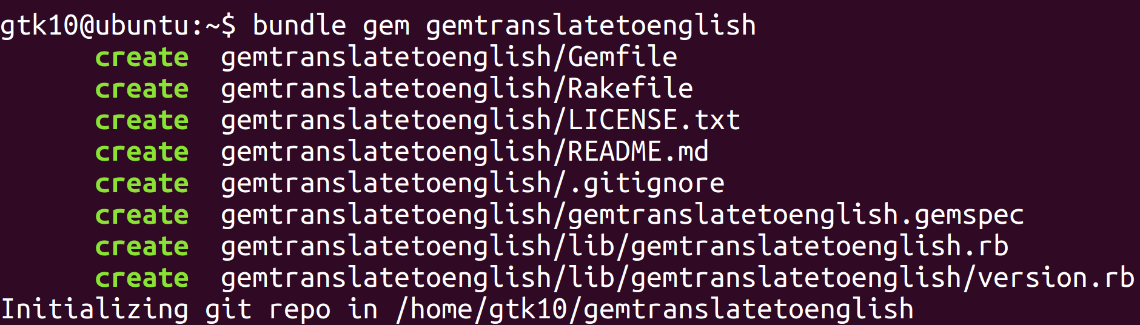
\includegraphics[scale=0.4]{images/execucao_que_cria_gema_gemtranslatetoenglish}
  \caption{Execução que cria gema gemtranslatetoenglish}
  \label{fig:execucao_que_cria_gema_gemtranslatetoenglish}
\end{figure}
\end{comment}


\subsection{Gemspec}
\label{subsection:gemspec}

Agora que possuimos a estrutura da gema, devemos fazer a edição do arquivo \emph{\textbf{gemspec}}
para informar os dados básicos da gema, e isso pode ser feito editando o arquivo ‘‘ 'nome da gema'.gemspec ''.
No nosso exemplo, fizemos a edição do arquivo ‘‘gemtranslatetoenglish.gemspec'' resultado no arquivo mostrado
no código \ref{lst:gemspec_gemtranslatetoenglish}
%na imagem ‘‘Figura \ref{fig:gemspec_gemtranslatetoenglish} - gemspec gemtranslatetoenglish''
, onde cada linha será explicada com mais detalhes logo a seguir.

\lstinputlisting[ style=customBash, caption={gemspec gemtranslatetoenglish}, label={lst:gemspec_gemtranslatetoenglish}]
{codigos/gemtranslatetoenglish/gemtranslatetoenglish.gemspec}

\begin{comment}
\begin{figure}[ht]
  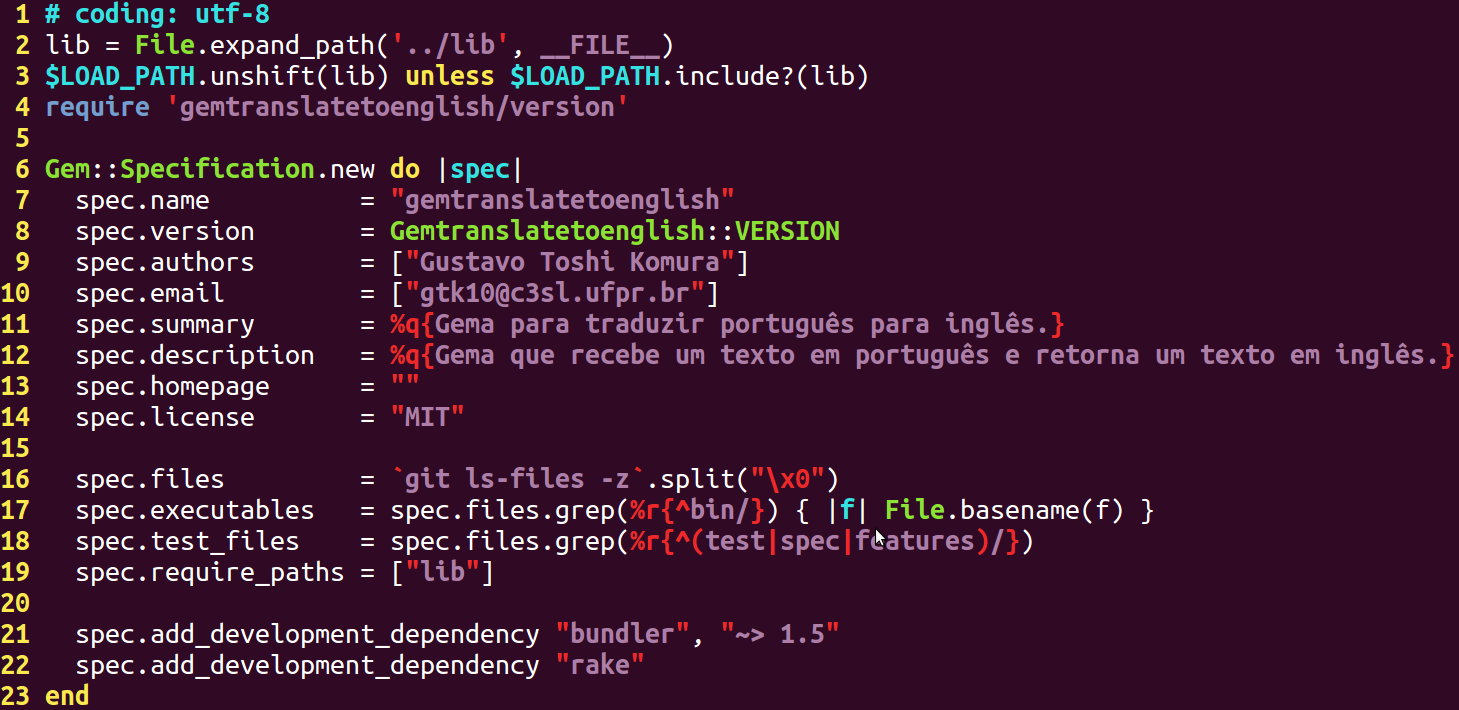
\includegraphics[scale=0.3]{images/gemspec_gemtranslatetoenglish}
  \caption{gemspec gemtranslatetoenglish}
  \label{fig:gemspec_gemtranslatetoenglish}
\end{figure}
\end{comment}

\begin{itemize}

 \item ‘‘\emph{\# coding: utf-8}'' na linha ‘‘1'' indica que o texto do arquivo está no formato \emph{UTF-8}.

 \item ‘‘\emph{lib = File.expand\_path('..\/lib', \_\_FILE\_\_)}'' na linha ‘‘2'' indica onde se encontra o
 diretório \emph{\textbf{lib}} da gema.

 \item ‘‘\emph{\$LOAD\_PATH.unshift(lib) unless \$LOAD\_PATH.include?(lib)}'' na linha ‘‘3'' faz o
 carregamento dos arquivos que estão no diretório \emph{\textbf{lib}}, somente se o diretório já
 esta definido.

 \item ‘‘ \emph{require 'gemtranslatetoenglish/version'} '' na linha ‘‘4'' requisita o arquivo de versão da
 gema.

 \item ‘‘\emph{Gem::Specification.new do |spec|} ... end'' da linha ‘‘6'' a ‘‘23'' define a especifação da
 gema como \emph{spec}, ou seja, ao invés de escrever ‘‘\emph{Gem::Specification}'' a todo momento que for
 definir uma especificação da gema se escreve somente ‘‘\emph{spec}''.

 \item ‘‘\emph{spec. }'' da linha ‘‘7'' a linha ‘‘14'' defini-se espcificações básicas da gema, como nome,
 versão, autor, e-mail do autor, breve descrição, descrição completa, página e tipo de licença.

 \item ‘‘\emph{spec.files = `git ls-files -z`.split("$\backslash$x0")}'' na linha ‘‘16'' indica os arquivos
 que devem ser incluídos na gema. Esses arquivos são incluídos dinâmicamente através do comando
 ‘‘\emph{git ls-files -z}''. Este comando do \emph{git}, traz como resultado todos os arquivos que estão
 naquele repositório, colocando entre as \emph{PATH}s, o caracter ‘‘\emph{$\backslash$0}''
 (\emph{line termination on output}). Por consequência, com a adição do comando \emph{Ruby}
 ‘‘\emph{.split("$\backslash$x0")}'', é feita a divisão por ‘‘\emph{$\backslash$0}'', separandos as
 \emph{PATH}s dos arquivos. Deste modo, os arquivos adicionados na gema, são todos que estão no repositório.

 Para se adicionar arquivos no repositório é necessário executar o comando ‘‘\emph{git add PATH}'',
 onde \emph{PATH} é o caminho do arquivo que se deseja adicionar no repositório.

 \item ‘‘\emph{spec.executables = ...}'' e ‘‘\emph{spec.tes\_files = ...}'' nas linhas ‘‘17'' e ‘‘18''
 indicam os arquivos executáveis e os arquivos de teste respectivamente. Também indica que os arquivos dentro
 destes diretórios, devem ter permissão de execução.

 \item ‘‘\emph{spec.require\_paths = ["lib"]}'' requisita o diretório da \emph{\textbf{lib}} da gema.

 \item ‘‘\emph{spec.add\_development\_dependency = ...}'' nas linhas ‘‘21'', ‘‘22'' e ‘‘23'' requistam como
 dependências as gemas ‘‘\emph{bundle}'' versão ‘‘1.5'', ‘‘\emph{rake}'' e ‘‘\emph{action\_controller}''
 respectivamente.

\end{itemize}


\subsection{Desenvolvimento de código de funcionalidade ou teste}
\label{subsection:desenvolvimento_de_codigo_de_funcionalidade_ou_teste}

Nesse momento podemos tomar 2 caminhos e isso depende da metodologia de projeto que adotadomos no inicio
do desenvolvimento, ou seja, é nesse momento que podemos desenvolver o código das funcinalidades
ou implementar o código de testes.

Na metodologia tradicional se faz a implementação do código de funcionalidades e depois se
desenvolve o código para testar as funcionalidades. Por outro lado, na metodologia voltada para
testes, se implementa o código de testes para depois se desenvolver o código de funcionalidades.

Seguindo a metodologia tradicional, primeiramente iremos fazer o código das funcinalidades da gema.
Depois ao terminar de criar essas funcionalidades, iremos elaborar os arquivos testes, mas nada o impede
de desenvolver os códigos de testes que serão apresentado na sub-seção
\ref{subsection:codigo_de_teste_no_diretorio_test_ou_spec}, antes de desenvolver os códigos de funcionalidade
mostrados na sub-seção \ref{subsection:codigo_de_funcionalidade_no_diretorio_lib}.

\subsection{Código de Funcionalidade no Diretório Lib}
\label{subsection:codigo_de_funcionalidade_no_diretorio_lib}

Nesta sub-seção vamos aprender a fazer o código de funcionalidade de uma gema, mas caso deseje fazer
primeiro os códigos de casos de testes, pode-se consultar a sub-seção
\ref{subsection:codigo_de_teste_no_diretorio_test_ou_spec}, e depois retornar para esta sub-seção para dar
continuidade ao desenvolvimento.

Caso esse código de funcionalidade seja desenvolvido por meio de código \emph{Ruby}, devemos fazer a
edição e a criação de arquivos no diretório \emph{\textbf{lib}}. Este diretório obrigatoriamente deve
possuir um arquivo ‘‘ 'nome da gema'.rb '' e um diretório, com um arquivo de versão, também com o
nome da gema. No nosso exemplo, podemos verificado no código
\ref{lst:execucao_que_cria_gema_gemtranslatetoenglish}, que após a execução do comando
‘‘\emph{bundle gem gemtranslatetoenglish}'', é feita a criação do arquivo
‘‘\emph{lib/gemtranslatetoenglish.rb}'' na linha ‘‘8'', e a criação do drietório
‘‘\emph{lib/gemtranslatetoenglish}'' com o arquivo ‘‘\emph{version}'' na linha ‘‘9''.

O arquivo ‘‘\emph{version}'', somente define a versão que a gema está. No nosso exemplo da gema
‘‘\emph{gemtranslatetoenglish}'', a primeira versão é a ‘‘\emph{0.0.1}''.

Basicamente a descrição da versão de uma gema é uma string com números e pontos. Também é permitido
colocar ao final a palavra chave ‘‘\emph{pre}'', caso seja um pré-lançamento de alguma versão.
Por exemplo, ‘‘\emph{1.0.0.pre}'' é um pré-lançamento da versão ‘‘\emph{1.0.0}''.

O \emph{Rubygems} recomenda seguir as seguintes politicas mencionadas logo abaixo que foram consultadas
em \emph{\href{http://guides.rubygems.org/patterns/\#semantic-versioning}{semantic-versioning}}
\footnote{semantic-version: \url{http://guides.rubygems.org/patterns/\#semantic-versioning}} e em
\emph{\href{http://guides.rubygems.org/specification-reference/\#version}{specification-reference-version}}
\footnote{specification-reference-version: \url{http://guides.rubygems.org/specification-reference/\#version}}.

\begin{itemize}
 \item PATH : “0.0.X” para pequenas alterações, como por exemplo correção de pequenos \emph{bugs}.
 \item MINOR: “0.X.0” para médias alterações, como por exemplo alteração/adição de funcionalidades.
 \item MAJOR: “X.0.0” para grandes alterações, como por exemplo remoção de alguma funcionalidade.
\end{itemize}

Antes de iniciarmos a codificação das funcionalidades da gema, precisamos entender algumas diferenças
básicas de conceitos do \emph{Ruby}, como por exemplo a diferença entre \emph{module} e \emph{class},

Os ‘‘\emph{modules}'' ou módulos se preferir, definem um conjunto de métodos e constantes. Podemos
dizer que os métodos dos módulos são estáticos, pois não precisamos instanciar o módulo para usar os
seus métodos. Contudo podemos dizer que os módulos são parecidos com o conceito de interface do
\emph{Java}.

Por outro lado a ‘‘\emph{class}'' também é um conjunto de métodos e constantes, no
entanto para usar os seus métodos e constantes é necessário instância-lá, ou seja, é necessário criar
um objeto da ‘‘\emph{class}'' na memória para usar os seus respectivos métodos.

Contudo por essas características podemos dizer que uma ‘‘\emph{class}'' é basicamente
uma subclasse do ‘‘\emph{module}'', pois a ‘‘\emph{class}'' possui 4 métodos a mais, que no caso são
os métodos ‘‘\emph{initialize()}'', ‘‘\emph{superclass()}'', ‘‘\emph{allocate()}'' e ‘‘\emph{to\_yank()}''.

Agora que temos alguns conceitos do \emph{Ruby} apresentados, podemos continuar com a implementação
da nossa gema.

No arquivo ‘‘ lib/'nome da gema'.rb '' temos a possibilidade de escerver todas as
funcinalidades desejadas. No nosso exemplo o arquivo ‘‘lib/gemtranslatetoenglish.rb'' é mostrado no código
\ref{lst:gemtranslatetoenglish.rb}, onde cada linha é explicado
logo a seguir.

\lstinputlisting[ style=customRuby, caption={gemtranslatetoenglish.rb}, label={lst:gemtranslatetoenglish.rb}]
{codigos/gemtranslatetoenglish/lib/gemtranslatetoenglish.rb}

\begin{itemize}

 \item ‘‘\emph{require "gemtranslatetoenglish/version"} '' na linha ‘‘1'' é feita a requsição do arquivo de
 versão.

 \item ‘‘\emph{require "gemtranslatetoenglish/translatetoenglish.rb"} '' na linha ‘‘2'' é feita a requisição
 do arquivo ‘‘\emph{translatetoenglish.rb}'' contido no diretório ‘‘gemtranslatetoenglish''.

 \item ‘‘\emph{module Gemtranslatetoenglish ... end}'' na linha ‘‘4'' a ‘‘6'' define o módula da gema.

 \item ‘‘\emph{ActionController::Base.helper Gemtranslatetoenglish::Helpers::Translatetoenglish}'' na linha
 ‘‘8'' define uma extensão da classe ‘‘\emph{ActionController::Base.helper}'', onde a classe a ser
 acrescentada é a classe ‘‘\emph{Gemtranslatetoenglish::Helpers::Translatetoenglish}''. Esta extensão foi
 adicionada para que no momento de uso das funcionalidades da gema na \emph{view} não fosse necessário
 fazer a chamada de tradução  escrevendo toda \emph{PATH}. Por exemplo para chamar a função de tradução,
 ao invés de chamar ‘‘\emph{gemtranslatetoenglish.Translatetoenglish.translate(‘Oi’)}'', se faz a chamada
 ‘‘\emph{translate(‘Oi’)}'' na \emph{view}. Isto é possível, pois nos projetos do
 \emph{framework Ruby On Rails}, os métodos de auxilio das \emph{view}, por simplificação já possuem a
 \emph{PATH} ‘‘\emph{ActionController::Base.helper}'' , deste modo, ao se incorporar um método nesta classe,
 não é mais necessário digitar a \emph{PATH} por completo.

\end{itemize}

Podemos perceber que o comando ‘‘\emph{require}'' é utilizado para fazer a chamada de código de outros
arquivos e isso serve para fazer a modularização da gema que no caso é uma boa prática de programação.
Suponha que desenvolvemos uma gema e depois de um certo tempo precisamos fazer a manutenção do
seu código. Neste caso se não modularizamos a gema, a correção de \emph{bugs} ou mesmo a adição de
novas funcionalidades, torna-se uma tarefa muito complexa, pois não existe nenhuma organização
estrutural na gema preparada para facilitar esse tipo de operação.

Observando novamente o código \ref{lst:gemtranslatetoenglish.rb}, podemos perceber que na linha ‘‘4''
foi feito o \emph{require} do arquivo ‘‘\emph{gemtranslatetoenglish/translatetoenglish.rb}'' que
será mostrado no código \ref{lst:translatetoenglish.rb}, e explicado logo a seguir.

\lstinputlisting[ style=customRuby, caption={translatetoenglish.rb}, label={lst:translatetoenglish.rb}]
{codigos/translatetoenglish_simplificado.rb}

\begin{itemize}

  \item ‘‘\emph{module ... end} nas linhas ‘‘1'', ‘‘2'' e ‘‘3'' define a árvore de módulos
  ‘‘\emph{Gemtranslatetoenglish}'' na raiz, ‘‘\emph{Helpers}'' no segundo nível e ‘‘\emph{Translatetoenglish}'' no
  terceiro.
  
  \item ‘‘\emph{def translate( phrase) ... end}'' da linha ‘‘5'' até a linha ‘‘34'', define
  a função de tradução da gema, onde foi definido somente duas traduções, ‘‘\emph{OI}''
  para ‘‘\emph{HELLO}'' e ‘‘MUNDO'' para ‘‘\emph{WORLD}''.

  A árvore definida no código \ref{lst:translatetoenglish.rb} foi necessário por causa do código
  inserido na linha ‘‘8'' ‘‘\emph{ActionController::Base.helper Gemtranslatetoenglish::Helpers::Translatetoenglish}''
  no código \ref{lst:gemtranslatetoenglish.rb} que serve para evitar a necesseidade de escrever a
  \emph{PATH} completa na \emph{view} para chamar uma função da gema na \emph{view}.

\end{itemize}


\subsection{Código de Teste no Diretório Test ou Spec}
\label{subsection:codigo_de_teste_no_diretorio_test_ou_spec}

Lembrando que podemos fazer o desenvolvimento de código de funcinalidades ou o código de testes, e isso é
dependente da metodologia adotada no inicio do projeto. Esta sub-seção tem o objetivo de mostrar como se pode
desenvolver o código de casos de testes, mas caso queira fazer o código de funcionalidade antes, se pode
consutar a sub-seção \ref{subsection:codigo_de_funcionalidade_no_diretorio_lib}.

Para se fazer os testes, deve-se criar os arquivos de testes dentro do diretório ‘‘\emph{test}'' ou se
preferir ‘‘\emph{spec}''. Não existe um padrão especificado, mais recomenda-se criar um arquivo de
teste com o nome ‘‘\emph{test/test\_‘definição do teste'.rb}''. No nosso exemplo, criamos o arquivo
‘‘\emph{test/test\_check\_translate.rb}'' no código \ref{lst:test_check_translate.rb},
explicado logo a seguir.

\lstinputlisting[ style=customRuby, caption={Testa translate gemtranslatetoenglish}, label={lst:test_check_translate.rb}]
{codigos/gemtranslatetoenglish/test/test_check_translate.rb}

\begin{itemize}

 \item Nas linhas ‘‘1'', ‘‘2'' e ‘‘3'' nos códigos ‘‘ \emph{require ‘...'} '' requisitamos respectivamente o
 ‘‘\emph{autorun}'' da gema ‘‘\emph{minitest}'' que utilizaremos para realizar os testes,
 ‘‘\emph{action\_controller}'' que utilizamos para evitar a obrigação de digitar a ‘‘\emph{PATH}'' completa
 na \emph{view}, e ‘‘\emph{gemtranslatetoenglish}'' que é a nossa gema de exemplo.

 \item Na linha ‘‘5'' fomos obrigados a fazer o ‘‘\emph{include}'' do módulo
 ‘‘\emph{Gemtranslatetoenglish::Helpers::Translatetoenglish}'' para que todas as funções deste módulo fossem
 disponiblizadas para uso. No nosso caso, era o método ‘‘\emph{translate()}''.

 \item Da linha ‘‘7'' a linha ‘‘16'' é definido a classe de teste ‘‘\emph{TranslateTest}'' que herda as
 características de ‘‘\emph{MiniTest::Unit::TestCase}''.

 \item Da linha ‘‘8'' a linha ‘‘11'' é definido o teste por palavra, onde é verificado através do
 ‘‘\emph{assert\_equal}'' se a ‘‘\emph{string}'' esperada no primeiro parâmetro é retornada pela chamada
 da função ‘‘\emph{Gemtranslatetoenglish::Helpers::Translatetoenglish.translate()}'' no segundo parâmetro.

 \item Da linha ‘‘12'' a linha ‘‘15'' é definido o teste por texto, onde é verificado através do
 ‘‘\emph{assert\_equal}'' se a ‘‘\emph{string}'' esperada no primeiro parâmetro é retornada pela chamada
 da função ‘‘\emph{Gemtranslatetoenglish::Helpers::Translatetoenglish.translate()}'' no segundo parâmetro.

\end{itemize}

Agora que temos o nosso arquivo de teste, precisamos criar o arquivo ‘‘\emph{Rakefile}''. Depois na pŕoxima
sub-seção \ref{subsection:execução_de_testes}, iremos explicar como realizar os teste com a execução da
ferramenta ‘‘\emph{rake}''.

No nosso exemplo da gema ‘‘\emph{gemtranslatetoenglish}'' desenvolvemos o seguinte arquivo
‘‘\emph{Rakefile}'' que pode ser visualizado no código \ref{lst:rakefile}, sendo explicado em detalhes
logo a seguir.

\lstinputlisting[ style=customRuby, caption={Rakefile gemtranslatetoenglish}, label={lst:rakefile}]
{codigos/gemtranslatetoenglish/Rakefile}

\begin{itemize}

\item Nas linhas ‘‘1'' e ‘‘2'' nos códigos ‘‘ \emph{require ‘...'} '' requisitamos respectivamente o
 ‘‘\emph{gem\_tasks}'' do ‘‘\emph{bundler}'' e ‘‘\emph{testtask}'' do ‘‘\emph{rake}'', ambos necessários para
 a execução dos testes.

 \item Da linha ‘‘4'' a ‘‘6'' é feito a criação de uma nova ‘‘\emph{task}'' de teste para cada arquivo
 que esteja no diretório ‘‘\emph{test}''.

 \item A linha ‘‘5'' com o código ‘‘ \emph{t.libs << ‘test'} '' inidica que os arquivos de testes estão no
 diretório ‘‘\emph{test}''.

 \item Por fim na linha ‘‘9'' com o código ‘‘\emph{task :default => :test}'', se requisita a execução
 dos testes.

\end{itemize}


\subsection{Execução de testes}
\label{subsection:execução_de_testes}

Esta sub-seção tem o objetivo de mostrar como se pode realizar os teste, após criar os códigos de
funcionalidade, visto na sub-seção \ref{subsection:codigo_de_funcionalidade_no_diretorio_lib}, e os códigos
de teste, visto na sub-seção \ref{subsection:codigo_de_teste_no_diretorio_test_ou_spec}.

Antes de realizarmos os testes, precisamos criar a gema com comando ‘‘\emph{gem build 'nome da gema'.gemspec}''
e fazer a instalação com o comando ‘‘\emph{sudo gem install 'nome da gema'-'versão da gema'.gem}''. No nosso
caso é fazer a criação e a instalação da gema ‘‘\emph{gemtranslatetoenglish}'', que pode ser feito da mesma
forma como no código \ref{lst:execucao_que_cria_e_instala_gemtranslatetoenglish}.

\lstinputlisting[ style=customBash, caption={Execução que Cria e Instala gemtranslatetoenglish}, label={lst:execucao_que_cria_e_instala_gemtranslatetoenglish}]
{codigos/execucao_que_cria_e_instala_gemtranslatetoenglish.sh }

Agora após ter implementado o código das funcionalidades, o arquivo de teste
‘‘\emph{test/test\_check\_translate.rb}'', o arquivo \emph{Rakefile}, e ter feito a criação e a instalação
da gema de exemplo, podemos realizar os testes com a execução do comando ‘‘\emph{rake}'' no terminal.

Com a execução dos testes, obtemos como resultado o código \ref{lst:execucao_rake_gema_gemtranslatetoenglish},
explicado logo a seguir.

\lstinputlisting[ style=customBash, caption={Execução rake gema gemtranslatetoenglish}, label={lst:execucao_rake_gema_gemtranslatetoenglish}]
{codigos/execucao_rake_gema_gemtranslatetoenglish.sh }

\begin{itemize}

 \item Na linha ‘‘1'' é feito a execução do comando ‘‘\emph{rake}'' para se realizar os testes.

 \item Na linha ‘‘5'' é mostrado que foram feitos 2 testes, no caso os 2 que definimos no código
 \ref{lst:test_check_translate.rb} nas linhas ‘‘8'' a ‘‘11'' no teste ‘‘\emph{test\_world\_translation}''
 e nas linhas ‘‘12'' a ‘‘15'' no teste ‘‘\emph{test\_text\_translation}''. Também é apresentado na
 linha ‘‘5'' que foram feitos 4 ‘‘\emph{assertions}'', no caso dois para cada caso de teste feitos por
 meio do ‘‘\emph{assert\_equal}''. E além disso é apresentado que não ocorreram  \emph{failures}'',
 ‘‘\emph{errors}'' e ‘‘\emph{skips}''.

\end{itemize}

Deste modo, ao se realizar estes testes garantimos que pelo menos a função ‘‘\emph{translate()}'' da gema
‘‘\emph{gemtranslatetoenglish}'', esta funcionando como o esperado.

Contudo no momento do desenvolvimento do código de testes, o aconselhável é para cada função adicionada
na gema, fazer testes com todas as possíveis entradas, verificando se o resultado para cada entrada
está correto.

Caso tenha mais interesse, existe a posibilidade de consultar o apêndice \ref{chapter:irb}, que mostra
como realizar testes com a ferramenta \emph{IRB}.


\subsection{Exemplo de uso de gemtranslatetoenglish}
\label{subsection:exemplo_de_uso_de_gemtranslatetoenglish}

Esta sub-seção tem o objetivo de mostrar a utilização da gema de exemplo ‘‘\emph{gemtranslatetoenglish}'',
que criamos no tutorial, em um projeto do \emph{framework Ruby On Rails}.

Até o momento falamos muito da utilização do \emph{action\_controller} para simplificar o uso da função
\emph{translate()} na \emph{view}, e agora vamos apresentar essa facilidade através de um exemplo,
fazendo o uso da gema ‘‘\emph{gemtranslatetoenglish}'' em um projeto.

O primeiro passo é criar um projeto no \emph{framework rails} e isso pode ser feito executando
o seguinte comando apresentado no código \ref{lst:executa_rails_new_para_gemtranslatetoenglish},
explicado logo a seguir.

\lstinputlisting[ style=customBash, caption={Executa rails new para gemtranslatetoenglish}, label={lst:executa_rails_new_para_gemtranslatetoenglish}]
{codigos/executa_rails_new_para_gemtranslatetoenglish_simplificado.sh}

\begin{itemize}

 \item O comando ‘‘\emph{rails new}'' implica na criação de um projeto básico do \emph{Ruby On Rails}.

 \item O nome ‘‘\emph{projeto\_teste\_gemtranslatetoenglish}'' é o nome do proejto a ser criado.

  \item Os códigos a partir da linha ‘‘2'' não representam execuções. No caso estes códigos somente
 mostram os passos realizados por causa da execução do comando na primeira linha.

 \item A execução deste comando implica na criação de alguns diretórios e arquivos e por simplificação
 somente explicaremos aqueles que vamos utilizar neste exemplo:

  \subitem - ‘‘\emph{Gemfile}'' arquivo que contém as \emph{gemas} que são utilizadas no projeto.

  \subitem - ‘‘\emph{config/routes.rb}'' arquivos que possui as rotas utilizadas no projeto.

\end{itemize}

Agora que criamos o projeto, precisamos fazer a criação de pelo menos um \emph{controller} e uma \emph{view}.
O \emph{controller} serve para receber uma requisição e determinar a partir dos parâmetros desta
requisição, a \emph{view} e os dados que devem ser apresentados. A \emph{view} serve para
determinar um formato e mostrar os dados no \emph{browser}.

Para o nosso exemplo, criamos o \emph{controller} ‘‘traducao'' e a \emph{view} ‘‘index'', com a execução do
comando que pode ser visto no código \ref{lst:executa_rails_generate_para_gemtranslatetoenglish},
explicado logo a seguir.

\lstinputlisting[ style=customBash, caption={Executa rails generate para gemtranslatetoenglish}, label={lst:executa_rails_generate_para_gemtranslatetoenglish}]
{codigos/executa_rails_generate_para_gemtranslatetoenglish.sh}

\begin{itemize}

 \item Na linha ‘‘1'' é feito a execução do comando ‘‘\emph{rails generate controller traducao index}'' no
 terminal para gerar o \emph{controller} ‘‘\emph{traducao}'', e a \emph{view} ‘‘\emph{index}'' para
 ‘‘\emph{traducao}''.

 \item Os códigos a partir da linha ‘‘2'' não representam execuções. No caso estes códigos somente
 mostram os passos realizados por causa da execução do comando na primeira linha.

 \item Na linha ‘‘2'' foi criado o \emph{controller} com o nome ‘‘\emph{traducao\_controller.rb}''

 \item Na linha ‘‘3'' foi adicionado no arquivo ‘‘\emph{config/routes.rb} o método \emph{get} para a
 \emph{view} ‘‘\emph{traducao/index}''.

 \item Na linha ‘‘6'' foi criado a \emph{view} ‘‘\emph{traducao/index.html.erb}''.

\begin{comment}
 \item A partir da linha ‘‘7'' são criados os arquivos de teste funcional, os \emph{helpers}, e os
 \emph{assets}. Os \emph{assets} possuem códigos \emph{coffeescript} que depois vão se tornar
 \emph{javascript} e códigos \emph{scss} que depois vão se tornar \emph{css}.
\end{comment}

\end{itemize}


Agora para fazer o uso da nossa gema de exemplo em um projeto feito no \emph{Ruby On Rails}, basta fazer a
inclusão da gema no final do arquivo \emph{Gemfile} da mesma forma como mostrado no código
\ref{lst:adiciona_gemtranslatetoenglish_no_gemfile}.

 \lstinputlisting[ style=customRuby, caption={Adiciona gemtranslatetoenglish no Gemfile}, label={lst:adiciona_gemtranslatetoenglish_no_gemfile}]
{codigos/adiciona_gemtranslatetoenglish_no_gemfile}

Agora que a gema ‘‘\emph{gemtranslatetoenglish}'' já esta incluída no nosso projeto, podemos fazer o uso
dela em uma \emph{view} da mesma maneira como apresentada no código \ref{lst:exemplo_do_translate_na_view},
explicado logo a seguir.

\lstinputlisting[ style=customRubyHTML, caption={Exemplo do translate() na view}, label={lst:exemplo_do_translate_na_view}]
{codigos/projeto_teste_gemtranslatetoenglish/app/views/traducao/index.html.erb}

 \begin{itemize}

  \item As linhas ‘‘1'' e ‘‘2'' já existiam, pois foram criadas automaticamente após a execução do comando
  ‘‘\emph{rails generate controller traducao index}'', que mostramos no código
  \ref{lst:executa_rails_generate_para_gemtranslatetoenglish}.

  \item Na linha ‘‘3'' inserimos uma \emph{tag <p>} indicando para o \emph{browser} que vamos inserir um
  texto. Depois inserimos a \emph{tag <\%= ... \%>} que indica que entre essas \emph{tags} será inserido um
  código \emph{Ruby}. E dentro destas \emph{tags}, chamamos o nosso método \emph{translate()} da gema
  ‘‘\emph{gemtranslatetoenglish}'' com o parâmetro ‘‘Oi Mundo''.

 \end{itemize}

Agora que temos a nossa função ‘‘\emph{translate()}'' dentro da \emph{view} ‘‘\emph{traducao/index}'', podemos
verificar se a tradução funciona corretamente. Para isso devemos dentro do diretório do nosso projeto,
iniciar o servidor no terminal através do comando ‘‘\emph{rails server -p2342}'', onde o parâmetro ‘‘-p2342''
indica que o servidor vai usar a porta ‘‘2342''.

Depois com o servidor funcionando, podemos verificar na imagem \ref{fig:resultado_de_translate_na_view}
que ao se acessar o endereço ‘‘localhost:2342/traducao/index'' no \emph{browser}, a nossa função de
tradução funciona corretamente, pois na página é apresentado o texto ‘‘HELLO WORLD''.

 \begin{figure}[ht]
  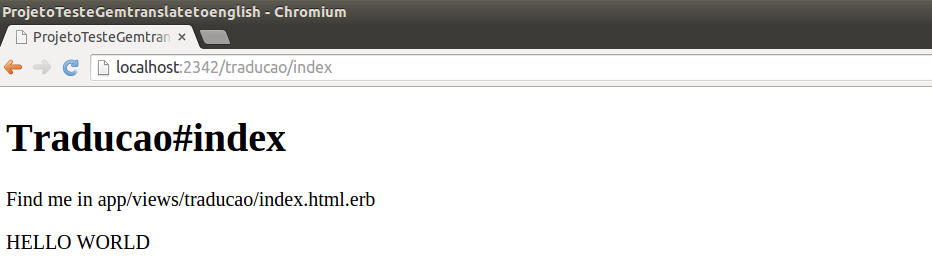
\includegraphics[scale=0.49]{images/resultado_de_translate_na_view.png}
  \caption{Resultado de Translate na View}
  \label{fig:resultado_de_translate_na_view}
\end{figure}
